\chapter{Results}

\section{Cohort of patients}

% TLCR
% Patients were followed from their diagnosis of stage IV disease.

% CCLM
% A total of 54 samples were obtained from 52 NSCLC patients and two healthy donors, after signing the appropriate informed consent.

% TESIS estela
% Para establecer la mejor estrategia metodológica, para la identificación del paciente candidato a recibir un inhibidor de ALK, se emplearán 20 muestras pre-tratamiento, pareadas de plasma y plaquetas, de pacientes con cáncer de pulmón no microcítico con enfermedad avanzada y translocación de ALK documentada según los protocolos asistenciales. Estas muestras se encuentran disponibles en el Biobanco del Hospital Universitario Puerta de Hierro.
% A fin de evaluar la utilidad de la biopsia líquida para monitorizar al paciente con translocación de ALK se reclutarán 30 pacientes, a razón de 15 pacientes por año. De cada paciente se recogerán muestras a los 2, 4, 6, 8, 12, 15 y 18 meses de tratamiento y a la progresión.
% % Los datos demográficos, clínico-patológicos, el estado mutacional del tumor, así como el estado funcional de los pacientes fueron obtenidos de los informes médicos. El ajuste de dosis y el cambio de medicación fueron documentados a lo largo del estudio.
%VARIABLES
% -Progresión de la enfermedad según criterios RECIST.
% -Supervivencia libre de progresión desde el inicio del tratamiento.
% -Supervivencia global desde el inicio del tratamiento.
% -Tasa de respuesta obtenida
% -Status EML4-ALK (positivo o negativo) en la biopsia líquida.
% -Niveles plasmáticos de EML4-ALK

% ALK paper
% In total, 33 plasma and 2 cerebrospinal fluid (CSF) specimens were collected and analyzed. Samples were collected at the time of disease progression which was assessed according to RECIST criteria v.1. 

\newpage

\section{Implemented Pipeline}

The development of the bioinformatic pipeline was divided into two steps: the implementation of the filtering algorithm itself; and that of a graphical interface to simplify the process of selecting parameters and saving the filtered variants.

\subsection{Algorithm Characterization}

In order to detect all variants at the ALK gene locus, specific conditions for each type of them have been established from a set of previously validated samples. The flow chart in \autoref{fig:Algorithm} represents the basic structure of the developed pipeline and the selection criteria based on certain variables as presented in the \textit{non-filtered-oncomine.tsv} file.

\begin{figure}[ht]
    \centering
    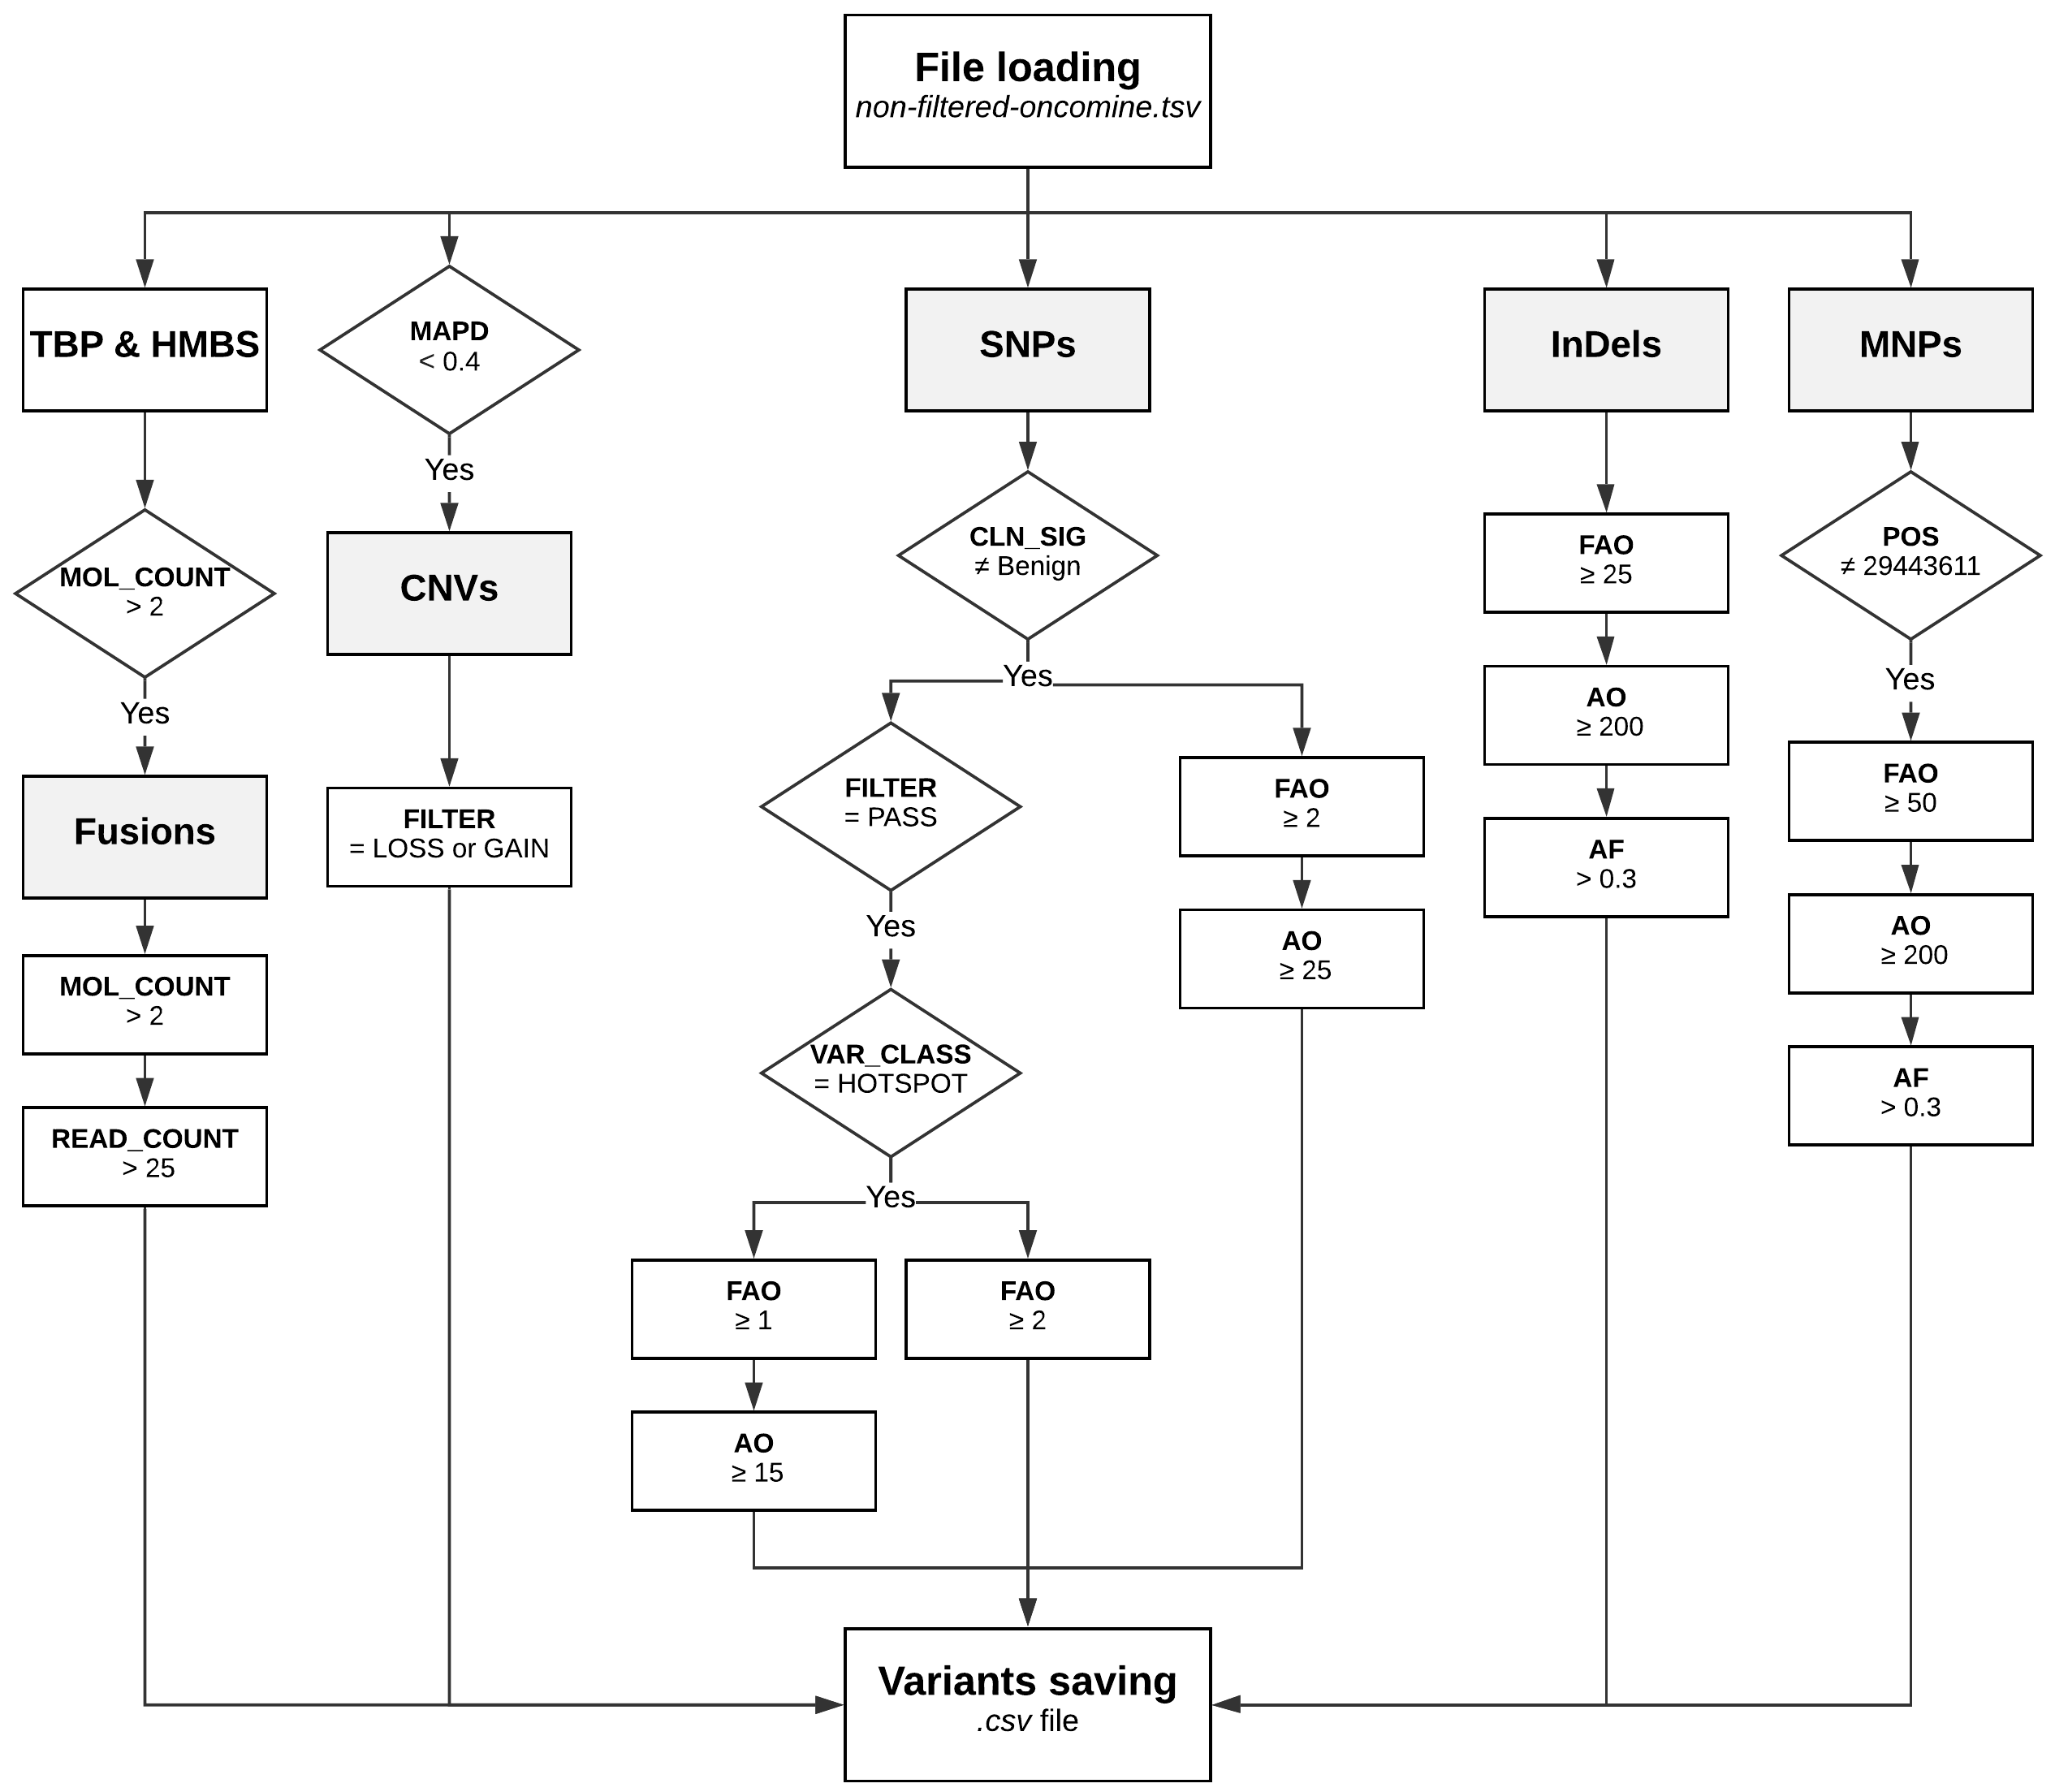
\includegraphics[width=\textwidth]{Images/chapter_4/mut_filtering.png}
    \caption{Flowchart of the bioinformatic pipeline optimized for the processing and assessment of variants at the ALK gene locus.}
    \label{fig:Algorithm}
\end{figure}

\subsubsection{Fusions Filtering}

The fusions filter selects translocations at the ALK locus with molecular coverage (MOL\_COUNT) $>$ 2 and fusion reads (READ\_COUNT) $>$ 25. On the other hand, two control genes are included in each sequencing process to measure the transcript abundance, TATA-binding protein (TBP) and hydroxymethylbilane synthase (HMBS). Both must have a molecular coverage (MOL\_COUNT) $>$ 2 to validate the filtered fusion variants by ensuring the correct amplification of them.

\subsubsection{Copy-Number Variations Filtering}

Following the Ion Reporter\texttrademark{} recommendations, to make a CNV call, the median of the absolute values of all pairwise differences (MAPD) must be $<$ 0.4. MAPD measures the absolute difference between the $log_2$ copy number ratios of adjacent amplicons and then calculates the median across all wells (\autoref{eq:MAPD}). Larger MAPD values indicate lower coverage uniformity and greater noise, resulting in a higher probability of erroneous CNV calls. Therefore, only samples showing a MAPD $<$ 0.4 were considered in further analysis, which consisted of selecting (FILTER) copy loss and gain in the ALK gene.
\begin{align} \label{eq:MAPD}
    MAPD &= median(\mid x_{i+1}-x_i \mid) \\
    \text{where}~  
    x_i &\equiv \text{$log_2$ ratio for marker i} \notag
\end{align}

\subsubsection{Single-Nucleotide Polymorphisms Filtering}


\subsubsection{Insertions and Deletions Filtering}


\subsubsection{Multiple-Nucleotide Polymorphisms Filtering}


% Algorithm

% Finally, the get.mutations() filter selects non-benign/likely-benign, single-nucleotide polymorphisms (SNPs), multi- nucleotide polymorphisms (MNPs), and indels in ALK locus. According to our data false positive are less likely in SNPs and very likely in MNPs. For this reason, the algorithm makes a positive call as long as any of the following 5 conditions is met:
% 1. SNPs in HotSpot file that have passed the Oncomine Variants 5.10 filter and that were detected in at least 1 molecular count with ≥15 reads (Rowtype=“SNP”; INFO.A.FAO≥1; INFO.A.AO ≥15; FILTER= “PASS”; FUNC1.oncomineVariantClass="Hotspot");
%2. SNPs that have passed the Oncomine Variants (5.10) filter and that were detected in at least 2 molecular counts (Rowtype= “SNP”; INFO.A.FAO ≥2; FILTER= “PASS”; FUNC1.oncomineVariantClass= "Hotspot”);
%3. SNPs that have been detected in at least 2 molecular counts with ≥25 reads (Rowtype= “SNP”; INFO.A.FAO ≥2; INFO.A.AO ≥25); 
%4. Variants different from MNPs that have been detected in at least 25 molecular counts with ≥25 reads and AF≥0.03 (Rowtype≠ “mnp”; INFO.A.FAO ≥25; INFO.A.AO ≥200; INFO.A.AF >0.03); and
%5. All variants that have been detected in at least 50 molecular counts with ≥200 reads and an AF≥ 0.03, excluding the position chr2:29443611 in ALK locus, which involves 6 consecutive guanines (G) (INFO.A.FAO≥50; INFO.A.AO≥200:  INFO.A.AF >0.03; POS≠ “29443611”).


% PAPER ALK
%Briefly, get.fusions() filter selects fusion variants involving ALK gene with >0 reads; get.CNVs() filter selects copy loss and gain in ALK gene; and get.positives() filter selects non-benign/likely-benign single-nucleotide polymorphisms (SNPs), multi- nucleotide polymorphisms (MNPs) and insertions and deletions insertions or deletions (InDels) in ALK gene as long as they meet any of the following 5 conditions: 
%1. Hotspot SNPs that have passed the Oncomine Variants (5.10) filter and that were detected in at least 1 molecular count with ≥15 reads; 
% 2. Hotspot SNPs that have passed the Oncomine Variants (5.10) filter and that were detected in at least 2 molecular counts; 
% 3. SNPs that have been detected in at least 2 molecular counts with ≥25 reads;
% 4. Variants ≠ MNPs that have been detected in at least 25 molecular counts with ≥25 reads and a minor allele frequency equal to or higher than 0.03; and 
% 5. All variants that have been detected in at least 50 molecular count with ≥200 reads and a minor allele frequency equal to or higher than 0.03, excluding 29443611 ALK position, which involves 6 guanines (G) attached. 

% NGS se equivoca más con los indles

\subsection{Graphical User Interface (GUI)}



\section{Statistic Analysis}

% Análisis estadístico
% Los resultados de frecuencia se expresarán en términos absolutos, en porcentajes e intervalos de confianza y, las variables cuantitativas como media ± desviación estándar o mediana (rango) según proceda.
% Para evaluar la concordancia del status de la translocación (positivo/negativo) entre las muestras de sangre (plaquetas y plasma) pre-tratamiento y el tejido se empleará el coeficiente Kappa de Cohen y su intervalo de confianza. Además, se analizará la sensibilidad, especificidad, valor predictivo positivo y valor predictivo negativo de la detección de la translocación en plasma (exosomas) y plaquetas, tomando como gold standar el resultado del tejido.
% Para analizar los datos de supervivencia de los pacientes se tomará como fecha de inicio, la fecha de inicio al tratamiento en primera línea y se recabarán los datos de: fecha de progresión, de muerte o fecha de última visita al oncólogo. La supervivencia libre de progresión se calculará desde la fecha de inicio al tratamiento en primera línea. Para el análisis de PFS y SG se usará el método de Kaplan-Meier y como estadístico de contraste se usará el Log- Rank. Los valores de los HR obtenidos serán ajustados por las variables clínico-patologícas pertinentes.
%Las pruebas con un valor de p <0.05 serán consideradas estadísticamente significativas.